\documentclass{templateNote}
\usepackage{tcolorbox}
\usepackage{hyperref}
\usepackage{amsmath}
\usepackage{amssymb}
\usepackage{soul}
\usepackage{circuitikz}
\usepackage{enumitem}
\usepackage{comment}
\usepackage{tikz}
\usepackage{parskip}
\usepackage{adjustbox}
\usepackage{booktabs}
\usepackage{tabularx}
\usepackage{array}
\usepackage{float}
\usepackage[utf8]{inputenc}
% \usepackage[table,xcdraw]{xcolor}
\usepackage{forest}
\usetikzlibrary{decorations.pathreplacing} % Para el corchete decorado
\usepackage[absolute,overlay]{textpos}


\begin{comment}
    \begin{textblock}{5}(10, 10)
        \begin{tcolorbox}[colback=green!5!white,colframe=green!75!black,title=Valor actual neto (VAN)]
            \begin{center}
                \begin{equation*}
                    VAN = \sum_{t=0}^{n} \frac{F_t}{(1+i)^t} - I_0
                \end{equation*}
            \end{center}
        \end{tcolorbox}
    \end{textblock}
\end{comment}

\definecolor{darkorange}{rgb}{0.8, 0.4, 0.0}


\begin{document}
\imagenlogoU{img/logoNGMFormal_sinF.png}
\linklogoU{https://github.com/NicoGomezM} 
% \imagenlogoD{img/logo-ubb-txt-face.png} 
\titulo{Apunte}
\asignatura{Formulación y Evaluación de Proyectos}
\autor{
    \indent
    Nicolás {Gómez Morgado}
}


\portada
\margenes 
\tableofcontents
\newpage

\section*{Importante}

\begin{itemize}
    \item Es necesario saber calcular porcentajes y tasas de interés, asi como también saber calcular el valor presente y futuro de una inversión.
    \item Es necesario saber calcular el Reajuste dados los valores que se nos entregan.
\end{itemize}

\subsection*{Conceptos clave}

\begin{itemize}
    \item \textbf{Proyectos:} Conjunto de actividades interrelacionadas que se realizan para alcanzar un objetivo.
    \item \textbf{Inversión:} Es el desembolso de recursos financieros para la adquisición de bienes y servicios.
    \item \textbf{Rentabilidad:} Es la relación entre los beneficios obtenidos y los recursos invertidos.
\end{itemize}

\newpage
\section{Criterios para evaluar inversiones}
\subsection{Método de evaluación inicial}
\begin{enumerate}[label=\alph*)]
    \item Incluir \textbf{todos los flujos de caja} que ocurren durante la vida del proyecto.
    \begin{center}
        \begin{tikzpicture}
            % Línea de tiempo
            \draw[-] (0,0) -- (10,0);
        
            % Etiquetas
            \node at (0,0.5) {Cuna};
            \node at (10,0.5) {Tumba};
        
            % Marcadores
            \draw (0,0.1) -- (0,-0.1);
            \draw (10,0.1) -- (10,-0.1);
        \end{tikzpicture}
    \end{center}
    \item Considerar el \textbf{valor del dinero} en el tiempo. \\
    Esto se refiere a que el dinero hoy vale más que el dinero en el futuro. Este termino se relaciona casi por completo con el costo de oportunidad.
    \item Incorporar la \textbf{tasa de retorno requerida} en el proyecto.\\
    Se refiere a que el rendimiento económico que promete el proyecto supere mínimamente al rendimiento que generalmente se ofrece por el mercado (métodos de inversion en banca).
\end{enumerate}

\subsection{Criterios comúnmente usados}

\subsubsection{Periodos de recuperacion de inversion (\textit{Payback})}
\begin{itemize}
    \item Numero de años que se requieren para recuperar la inversión inicial.
    \item Tiempo que le toma al proyecto generar suficientes ingresos para autofinanciarse.
    \item Depende de la naturaleza del proyecto y del criterio de los inversionistas determinar si el periodo de recuperación es aceptable. 
\end{itemize}
\textbf{Debilidades:}
\begin{itemize}
    \item \hl{Subjetivo}.
    \item No considera el valor del dinero en el tiempo.
    \item No considera la tasa de retorno requerida.
    \item No considera los flujos de caja después del periodo de recuperación.
\end{itemize}

\subsubsection{Periodo de recuperacion de inversion descontado (\textit{Payback descontado})}
\begin{itemize}
    \item Se calcula descontando los flujos de caja futuros a una tasa de descuento.
    \item Periodo de recuperación se calcula con los flujos netos.
\end{itemize}
\textbf{Debilidades:}
\begin{itemize}
    \item Dependen del criterio del inversionista.
\end{itemize}

\newpage

\begin{tcolorbox}
    \begin{center}
        
\begin{tikzpicture}
            % Lista de métodos
            \node[anchor=west] (van) at (0,0) {\textbf{• VAN}};
            \node[anchor=west] (ir) at (0,-0.5) {\textbf{• IR}};
            \node[anchor=west] (tir) at (0,-1) {\textbf{• TIR}};
        
            % Corchete
            \draw[decorate,decoration={brace,amplitude=10pt,mirror,raise=5pt},yshift=0pt] (3,0.5) -- (3,-1.5) node [black,midway,xshift=0.8cm] {};
        
            % Características
            \node[anchor=west] at (2.5,-0.5) {
                \begin{minipage}{0.65\textwidth}
                    \begin{itemize}
                        \item Considera todos los flujos de caja del proyecto.
                        \item Considera el valor del dinero en el tiempo.
                        \item Considera la tasa de retorno requerida.
                    \end{itemize}
                \end{minipage}
            };
        \end{tikzpicture}
    \end{center}
\end{tcolorbox}


\subsubsection{Valor actual neto (VAN)}

\begin{align*}
    VAN &= \sum_{t=0}^{n} \frac{\textnormal{FCA}_t}{(1+k)^t} - I_0
\end{align*}

\textbf{Criterios de decisión:}
\begin{itemize}
    \item Si $VAN > 0$, el proyecto es \textbf{aceptable}.
    \item Si $VAN < 0$, el proyecto es \textbf{rechazable}.
\end{itemize}

\subsubsection{Indice de Rentabilidad (IR)}

\begin{align*}
    IR &= \sum_{t=0}^{n} \frac{\textnormal{FCA}_t}{(1+k)^t}/I_0
\end{align*}

\textbf{Criterios de decisión:}
\begin{itemize}
    \item Si $IR \geq 1$, el proyecto es \textbf{aceptable}.
    \item Si $IR < 1$, el proyecto es \textbf{rechazable}.
\end{itemize}

\subsubsection{Tasa interna de retorno (TIR)}

\begin{align*}
    I_0 &= \sum_{t=0}^{n} \frac{\textnormal{FCA}_t}{(1+TIR)^t}
\end{align*}

\textbf{Criterios de decisión:}
\begin{itemize}
    \item Si $TIR > k$, el proyecto es \textbf{aceptable}.
    \item Si $TIR < k$, el proyecto es \textbf{rechazable}.
\end{itemize}

\newpage
\textbf{Ejemplo 1:} Una empresa estudia la posibilidad de emprender un proyecto de inversión de dos años de duración. El proyecto exige la compra de un activo con un desembolso inicial de \$86.000 . Con la actividad que genera dicho activo se esperan unos flujos de caja de \$45.000 el primer año y \$51.000 el segundo año. Se sabe que el tipo de interés del capital o coste del capital es del 6\% anual. Se pide:
\begin{enumerate}[label=\alph*)]
    \item Calcule la Tasa Interna de Retorno (TIR) de la inversión.
    \begin{align*}
        \frac{45000}{(1+TIR)} + \frac{51000}{(1+TIR)^2} &= 86000 \\
        86000 - \frac{45000}{(1+TIR)} - \frac{51000}{(1+TIR)^2} &= 0 \\
        \frac{86000(1+TIR)^2 - 45000(1+TIR) - 51000}{(1+TIR)^2} &= 0 \\
        \frac{86000(1+TIR)^2 - 45000 - 45000TIR - 51000}{(1+TIR)^2} &= 0 \\
        \frac{86000(1+2TIR+{TIR}^2)-45000TIR-96000}{(1+TIR)^2} &= 0 \\
        -10000 + 127000TIR + 86000{TIR}^2 &= 0 \\
        86000{TIR}^2 + 127000TIR - 10000 &= 0 \\
        86{TIR}^2 + 127TIR - 10 &= 0 
    \end{align*}
        \textbf{Resolviendo la ecuación cuadrática:}
    \begin{align*}
        TIR &= \frac{-b \pm \sqrt{b^2 - 4ac}}{2a} \\
        TIR &= \frac{-127 \pm \sqrt{127^2 - 4(86)(-10)}}{2(86)} \\
        TIR &= \frac{-127 \pm \sqrt{16129 + 3440}}{172} \\
        TIR &= \frac{-127 \pm \sqrt{19569}}{172} \\
        TIR &= \frac{12.8892}{172} = 0.07493 \wedge TIR = \frac{-265.8892}{172} = -1,5458 \\
        TIR &= 0.07493
    \end{align*}
    Por lo tanto la TIR es de 7.493\%.
    \item Calcule el VAN.
    \begin{align*}
        VAN &= \frac{45000}{(1+0.06)} + \frac{51000}{(1+0.06)^2} - 86000 \\
        VAN &= \frac{45000}{1.06} + \frac{51000}{1.1236} - 86000 \\
        VAN &= 42452.8301 + 45389.8184 - 86000 \\
        VAN &= 87842.6485 - 86000 \\
        VAN &= 1842.6485
    \end{align*}
    \item Explique si la inversión es aceptable según ambos criterios.
    \\Por lo tanto la inversion es aceptable ya que el VAN es positivo y la TIR es mayor al costo de oportunidad.
\end{enumerate}

\begin{tcolorbox}[colback=purple!5!white,colframe=purple!75!black,title=Importante]
    \begin{itemize}
        \item La TIR es buena herramienta siempre que los flujos sean convencionales. (-+++++...+)
        \item Con multiples cambios de signos se presentan varias TIR. (-++-++-+...+)
        \item La TIR \textbf{solo se usa} con flujos convencionales, en caso contrario se usa el \textbf{VAN}.
    \end{itemize}
\end{tcolorbox}

\textbf{Ejemplo:} Para una empresa con intereses del 15\% anual y con flujos de caja:

\begin{center}
    \begin{tikzpicture}
        % Línea de tiempo
        \draw[->] (0,0) -- (12,0) node[right] {Tiempo};
    
        % % Puntos de tiempo (espaciados más)
        % \foreach \x in {0, 2, 4, 6, 8, 10}
        %     \draw (\x,0.1) -- (\x,-0.1) node[below] {$\x$};
    
        % Flujos de caja (ajustados a los nuevos puntos de tiempo)
        \draw (0,0) -- (0,-0.5) node[below] {(900)};
        \draw (2,0) -- (2,0.5) node[above] {300};
        \draw (4,0) -- (4,0.5) node[above] {400};
        \draw (6,0) -- (6,0.5) node[above] {400};
        \draw (8,0) -- (8,0.5) node[above] {500};
        \draw (10,0) -- (10,0.5) node[above] {600};
    \end{tikzpicture}
\end{center}
Calcular:
\begin{enumerate}[label=\alph*)]
    \item TIR
    \item VAN
    \item IR
\end{enumerate}

\begin{align*}
    900 &= \frac{300}{1-TIR} + \frac{400}{(1-TIR)^2} + \frac{400}{(1-TIR)^3} + \frac{500}{(1-TIR)^4} + \frac{600}{(1-TIR)^5} \\
    &\textnormal{\textit{Calculo en excel:}}\\
    TIR &= 34,372\%
\end{align*}
Por lo tanto el TIR equivale a 34,372\%.

\begin{align*}
    VAN &= \frac{300}{(1+0.15)} + \frac{400}{(1+0.15)^2} + \frac{400}{(1+0.15)^3} + \frac{500}{(1+0.15)^4} + \frac{600}{(1+0.15)^5} - 900 \\
    &\textnormal{\textit{Calculo en excel:}}\\
    VAN &= 510,5161
\end{align*}
Por lo tanto el VAN equivale a 510,5161.

\begin{align*}
    IR &= (\frac{300}{(1+0.15)} + \frac{400}{(1+0.15)^2} + \frac{400}{(1+0.15)^3} + \frac{500}{(1+0.15)^4} + \frac{600}{(1+0.15)^5})/900 \\
    &\textnormal{\textit{Calculo en excel:}}\\
    IR &= 1,5672
\end{align*}

\begin{figure}[H]
    \centering
    \includegraphics[width=0.5\textwidth]{img/EjemploCalculo.png}
\end{figure}


\subsubsection{Tasa promedio de rendimiento (TPR)}

\begin{itemize}
    \item No considera flujos de caja.
    \item No considera el valor del dinero en el tiempo.
    \item Se basa en la utilidad contable promedio.
    \item Se usa porque es \textbf{fácil de calcular}.
\end{itemize}

\begin{align*}
    TPR &= \frac{\textnormal{Utilidad media}}{\textnormal{Inversión}} * 100
\end{align*}

\begin{tcolorbox}
    \begin{em}
        \begin{center}
            \begin{tabular}{l l}
                Ingresos por ventas & ~ \\
                Costo de ventas & \textcolor{red}{Deprec. y amortiz.} \\
            \end{tabular}
            \rule{11cm}{0.2 mm} \\[0.1 cm]
            \begin{tabular}{l l}
                Margen bruto & ~ \\
                Gastos de adm. y ventas & \textcolor{red}{Deprec. y amortiz.} \\
            \end{tabular}
            \rule{11cm}{0.2 mm} \\[0.1 cm]
            \begin{tabular}{l l}
                Resultado operacional & ~ \\
                Gastos financieros & ~ \\
            \end{tabular}
            \rule{11cm}{0.2 mm} \\[0.1 cm]
            \begin{tabular}{l l}
                Resultados antes de impuestos & ~ \\
                Impuestos a la renta & ~ \\
            \end{tabular}
            \rule{11cm}{0.2 mm} \\[0.1 cm]
            \begin{tabular}{l l}
                Resultado neto & ~ \\
                \textcolor{red}{+ Depreciación y amortización} & ~ \\
            \end{tabular}
            \rule{11cm}{0.2 mm} \\[0.1 cm]
            \begin{tabular}{l l}
                Flujo de caja & ~ \\
            \end{tabular}
        \end{center}
    \end{em}
\end{tcolorbox}

\textbf{Ejemplo:} Para una empresa que invierte \$900 y tiene los mismos flujos de caja que el ejercicio anterior, si esta inversion se deprecia en partes iguales en todos los periodos, calcular la TPR.

\begin{align*}
    TPR &= \frac{\frac{(300-(900/5)) + (400-(900/5)) + (400 -(900/5)) + (500 -(900/5)) + (600 -(900/5))}{5}}{900} \\
    TPR &= \frac{\frac{300-180 + 400-180 + 400-180 + 500-180 + 600-180}{5}}{900} \\
    TPR &= \frac{\frac{120 + 220 + 220 + 320 + 420}{5}}{900} \\
    TPR &= \frac{1300}{5*900} \\
    TPR &= \frac{1300}{4500} \\
    TPR &= 0.2888
\end{align*}

Por lo tanto la TPR es de 28,$\overline{88}$\%.

\rule{\linewidth}{0.1 mm}

\textbf{Ejercicio:} Una empresa tiene \$35000 dispuestos para inversiones, para las inversiones presentadas en la tabla, seleccionar los proyectos que se deben realizar basándose en su costo y VAN proporcionados.

\begin{center}
    \begin{tabular}{|c|c|c|}
        \hline
        Proyecto & Costo & VAN \\
        \hline
        A & 3600 & 380 \\
        B & 2100 & 500 \\
        C & 5800 & 1100 \\
        D & 7200 & 1060 \\
        E & 1060 & 320 \\
        F & 4490 & 1660 \\
        G & 2391 & 1010 \\
        H & 9810 & 2800 \\
        I & 6580 & 650 \\
        J & 1270 & 230 \\
        K & 1290 & 780 \\
        L & 5690 & 1270 \\
        \hline
    \end{tabular}
\end{center}

Conociendo el dinero enfocado en inversiones, se deben seleccionar los proyectos que se deben realizar basándose en su costo y VAN proporcionados. Se debe seleccionar los proyectos que tengan un VAN positivo y que no superen el monto total de la inversión, para hacer esto vamos a calcular el IR de cada proyecto.

\begin{center}
    \begin{tabular}{|c|c|c|c|}
        \hline
        Proyecto & Costo & VAN & IR \\
        \hline
        A & 3600 & 380 & 0.1055 \\
        B & 2100 & 500 & 0.2380 \\
        C & 5800 & 1100 & 0.1896 \\
        D & 7200 & 1060 & 0.1472 \\
        E & 1060 & 320 & 0.3018 \\
        F & 4490 & 1660 & 0.3704 \\
        G & 2391 & 1010 & 0.4223 \\
        H & 9810 & 2800 & 0.2853 \\
        I & 6580 & 650 & 0.0987 \\
        J & 1270 & 230 & 0.1811 \\
        K & 1290 & 780 & 0.6047 \\
        L & 5690 & 1270 & 0.2233 \\
        \hline
    \end{tabular}
\end{center}

Ahora con estos datos ordenaremos los proyectos de mayor a meno IR e iremos sumando sus costos para ver hasta que proyecto podemos llegar.

\begin{center}
    \begin{tabular}{|c|c|c|c|c|}
        \hline
        Proyecto & Costo & VAN & IR & Costo Acumulado\\
        \hline
        K & 1290 & 780 & 0.6047 & 1290 \\   
        G & 2391 & 1010 & 0.4223 & 3681 \\
        F & 4490 & 1660 & 0.3704 & 8171 \\
        E & 1060 & 320 & 0.3018 & 9231 \\
        H & 9810 & 2800 & 0.2853 & 19041 \\
        B & 2100 & 500 & 0.2380 & 21141 \\
        L & 5690 & 1270 & 0.2233 & 26831 \\
        C & 5800 & 1100 & 0.1896 & 32631 \\
        J & 1270 & 230 & 0.1811 & 33901 \\
        D & 7200 & 1060 & 0.1472 & 41101 \\
        A & 3600 & 380 & 0.1055 & 44701 \\
        I & 6580 & 650 & 0.0987 & 51281 \\
        \hline
    \end{tabular}
\end{center}

Por lo tanto los proyectos que se deben realizar son: K, G, F, E, H, B, L, C, J. No se utilizo el total de la inversion ya que para ninguno de los proyectos que quedaban alcanzaba el presupuesto.

\newpage
\section{Aspectos propios de un proyecto informático}
Dentro del desarrollo de proyectos informáticos, se deben considerar ciertos aspectos que son propios de este tipo de proyectos, los cuales son:

\subsection{Tipología de proyectos informáticos}
Los proyectos informáticos pueden ser clasificados en varios tipos dentro de los cuales están:

\begin{itemize}
    \item \textbf{Proyecto de desarrollo de aplicaciones:} Crear y poner en marcha programas o sistemas informáticos.
    \item \textbf{Proyectos de equipamiento:} Adquirir por primera vez equipos, dentro de estos incluyendo tanto HW como SW básico utilitario.
    \item \textbf{Proyectos de mejoramiento, ampliación o reposición:} Aumentar la capacidad y/o calidad de los servicios existentes.
\end{itemize}

\subsection{Ciclo de proyectos informáticos}
Guarda relación con el ciclo de vida de un proyecto, tomando en cuenta secciones utilizadas en el ciclo de vida tradicional (CVT):

\begin{itemize}
    \item \textbf{Diseño lógico:} Se define que tipo de sistemas se desarrollaran, que información es relevante para los sistemas, que procesaran los sistemas, etc.
    \item \textbf{Diseño físico:} Se define que tipos de archivos se utilizaran, que tipo de accesos, que tipo de lenguajes, etc.
    \item \textbf{Construcción:} Una vez diseñado el sistema, se procede a construirlo.
    \item \textbf{Implementación:} Se realizan pruebas, poblamiento de datos, marcha blanca y puesta en marcha.
    \item \textbf{Operación y mantenimiento:} Se mantiene el sistema en funcionamiento y se realizan las mejoras necesarias.
\end{itemize}

\subsection{Preparación de proyectos informáticos}
Para desarrollar un proyecto informático se debe tener en consideración ciertos puntos:

\begin{itemize}
    \item Identificación y definición del problema a resolver.
    \item Diagnostico de la situación actual.
    \item Descripción general de requerimientos.
    \item Programacion de actividades para la etapa de diseño.
    \item Requerimientos de personal para la etapa de diseño.
    \item Estimación de beneficios.
    \item Estimación de costos de inversion, operación y mantenimiento para la etapa de ejecución.
    \item Análisis de requerimientos para el diseño lógico.
    \item Alternativas de solución.
    \begin{itemize}
        \item Restricciones de cada alternativa.
        \item Producto o servicio de cada alternativa.
    \end{itemize}
    \item Evaluación y selección de alternativas.
    \item Atributos relevantes.
    \begin{itemize}
        \item Atributos imprescindibles (Atributos que deben cumplir todas las alternativas).
        \item Atributos evaluables (Atributos deseables y muy deseables).
    \end{itemize}
\end{itemize}

\subsubsection{Atributos imprescindibles}
Son aquellos atributos que deben cumplirse obligatoriamente en su totalidad. A lo menos deben considerarse:
\begin{itemize}
    \item La alternativa de solución esta de acuerdo con la política informática de la entidad.
    \item La institución cuenta con las capacidad es técnicas y administrativas para soportar la solución (HW, SW, personal, etc).
\end{itemize}

\subsubsection{Atributos evaluables}
Son aquellos medibles y que permiten evaluar las alternativas de solución y discriminar entre ellas, puesto que debe existir variabilidad y complejidad en las alternativas de solución. 

La clasificación de deseables y muy deseables debe formularse con base en el plan informático de la institución.

Se espera que los atributos hagan hincapié en la información (eficiencia, eficacia, confiabilidad, seguridad, etc).

\newpage
\subsubsection{Evaluacion de los atributos}
\begin{itemize}
    \item \textbf{Efectividad:} Capacidad de la alternativa para cumplir con los objetivos.
    \begin{table}[H]
        \centering
        \begin{tabular}{|>{\centering\arraybackslash}m{6cm}|c|c|c|c|}
            \hline
            \textbf{Funcionalidades del Sistema} & \textbf{Alt. 1} & \textbf{Alt. 2} & \textbf{  ...  } & \textbf{Alt. N} \\
            \hline
            \textcolor{darkorange}{\textbf{\textit{Muy deseables}}} & 100\% & 50\% & & 100\% \\
            Información en línea & 1 & 1 & & 1 \\
            Interfaces gráficas & 1 & 0 & & 1 \\
            \hline
            \textcolor{darkorange}{\textbf{\textit{Deseables}}} & 33\% & 100\% & & 33\% \\
            Emisión de cartas & 0 & 1 & & 0 \\
            Control de cambios & 1 & 1 & & 1 \\
            Otros atributos menores & 0 & 1 & & 0 \\
            \hline
        \end{tabular}
    \end{table}
    \item \textbf{Plataforma tecnológica:} Capacidad de la alternativa para soportar la solución.
    \begin{itemize}
        \item Confidencialidad.
        \item Integridad.
        \item Disponibilidad.
        \item Confiabilidad de la información.
        \item Información externa:
        \item la información debe ser apropiada para satisfacer los requerimientos de otras instituciones.
    \end{itemize}
    \item \textbf{Calidad técnica de la solución:} Capacidad de la alternativa para cumplir con los requerimientos técnicos.
    \begin{itemize}
        \item Seguridad.
        \item Disponibilidad.
        \item Portabilidad.
        \item Accesibilidad.
        \item Escalabilidad.
    \end{itemize}
    \item \textbf{Ahorro de costos operaciones:} Capacidad de la alternativa para reducir los costos operacionales.
    \begin{itemize}
        \item Variable muy importante para elegir entre las alternativas.
        \item Analizar partidas que generen ahorros.
        \item Lo importante es que sean objetivamente cuantificables.
        \item Deben expresarse en términos absolutos y relativos.
    \end{itemize}
\end{itemize}

\subsection{Situación sin proyecto}
Para poder desarrollar un proyecto informático, es necesario saber de antemano:
\begin{itemize}
    \item Descripción de la organización o entorno afectado por el proyecto.
    \item Descripción de la unidad o departamento.
    \item Presentación de la solución informática actual.
    \item Descripción de los procesos.
    \item Diagrama de flujo de datos que represente la situación actual.
\end{itemize}

\subsection{Mayores razones por las que un proyecto informático falla}\label{sec:razones-falla}


\begin{itemize}
    \item \textbf{Higher than expected maintenance fees (Mayor costo de mantenimiento al esperado):} El costo de mantenimiento es mayor al esperado.
    \item \textbf{Lack of governance (Falta de gobernanza):} No se tiene un plan de como desarrollar el proyecto.
    \item \textbf{Internal politics (Política interna):} Problemas respectivos a la política de la empresa que impiden la realización del proyecto.
    \item \textbf{Poor communication between business and IT(Comunicación pobre entre el negocio y la TI):} Falta de comunicación entre los departamentos de informática y negocios de la empresa.
    \item \textbf{Unclear expectations (Expectativas poco claras):} Las expectativas de lo que se espera que logre el proyecto no están bien definidas.
    \item \textbf{Lack of fact-based analysis (Falta de análisis basado en hechos):} No se tiene un análisis basado en hechos para la realización del proyecto.
    \item \textbf{Lack of input from users (Falta de aportes de los usuarios):} No hay suficiente apoyo de los usuarios a los que va dirigido el sistema para la población de datos o el desarrollo del proyecto.
    \item \textbf{Changes in project size, budget and scope (Cambios en el tamaño, presupuesto y alcance del proyecto):} Cambios en el proyecto que impiden que avance o alcance un punto de finalización.
    \item \textbf{Change in key personal (Cambio en personal clave):} Cambios en el personal clave del proyecto que son clave para el desarrollo del proyecto ya que manejan información que el personal nuevo no tiene.
    \item \textbf{Schedule overruns (Retrasos en el cronograma):} Debido a los problemas anteriores o la falta de planificación, el proyecto se retrasa.
\end{itemize}

\newpage
\section{Etapas de formulación y evaluación de un proyecto}

\subsection{Proyecto}
Se entiende por proyecto todo plan y disposición para ejecutar una inversion. El concepto anterior abarca desde el reemplazo de un activo hasta la creación de nuevos negocios.

En otras palabras un proyecto es una \textbf{actividad económica que busca acrecentar la riqueza de sus inversionistas}.

\subsection{Proyecto informático}
Plan que consiste en materializar una idea relacionada con equipamientos de hardware, software o comunicaciones (o combinaciones entre estos), con el fin de obtener un cierto resultado en un sistema de información.

\subsubsection{Objetivos de un proyecto informático}
\begin{itemize}
    \item \textbf{De servicio:} Lo que se espera del sistema del punto de vista del \textit{cliente/usuario}.
    \item \textbf{De producción:} Lo que se espera del sistema del punto de vista del \textit{departamento de informática} (costo, plazo, calidad, rendimiento, etc).
    \item \textbf{Estratégicos:} Lo que se espera del sistema del punto de vista de la \textit{dirección superior de la entidad}. Estos objetivos son de largo plazo y afectan a todas las areas (cobertura, integración, imagen, migración, etc.).
\end{itemize}

\subsection{Necesidad de evaluación de proyectos}
La evaluación de un proyecto surge de la necesidad de anticipar si generará pérdidas o ganancias y en qué medida. Esto permite determinar si es rentable asignarle recursos o si existen alternativas más favorables para su inversión.

Las evaluaciones de proyectos permiten identificar los flujos de caja esperados que con mayor probabilidad generara el proyecto.

\subsection{Evaluación de proyectos}
Pretende la medición objetiva de ciertas magnitudes cuantitativas resultantes del estudio del proyecto. Lo importante radica en que las premisas y supuestos que se hayan realizado se hayan sometido a convalidaron a traves de mecanismos y técnicas. Mientras mas precisas la estimación de ingresos y egresos, ademas del horizonte de vida del proyecto, más acertada sera su evaluación.

\subsubsection{Evaluacion social de proyectos}
En este tipo de evaluación se comparan los beneficios y costos que una inversion pueda significarle a la comunidad local, regional o nacional.

Mientras que \textbf{evaluación privada} utiliza precios de mercado, la \textbf{evaluación social} utiliza precios sociales. 

\subsection{Tipos de proyectos (según la finalidad de la inversión)}
\begin{itemize}
    \item Pra crear una nueva empresa.
    \item Para modernizar una empresa existente.
    \item Para evaluar gastos de mantenimiento.
    \item Para introducir mejoras (aumentar ingresos / ahorrar costos).
    \item Para ampliar la capacidad actual.
    \item Para lanzar nuevos productos.
    \item Para cumplir con las leyes y normativas vigentes.
\end{itemize}

\subsubsection{Magnitud de un proyecto informatico}
\begin{itemize}
    \item \textbf{Mantenimiento de programas:} Involucra solucionar fallas menores en un sistema, por omisiones en el diseño o errores en la programación.
    \item \textbf{Modificaciones en programas:} Cambios en la estructura de los programas.
    \item \textbf{Mejoramiento de sistemas:} Agregar nuevas funciones a un sistema existente.
    \item \textbf{Creación o reemplazo de sistemas:} Crear un nuevo sistema o reemplazar uno existente.
\end{itemize}

\subsection{Componentes de decisión de inversion}
\begin{itemize}
    \item \textbf{Desisor:} Persona que toma la decisión de invertir.
    \begin{itemize}
        \item Inversionista.
        \item Gerente.
        \item Financista.
        \item Evaluador.
    \end{itemize}
    \item \textbf{Variables controladas.}
    \item \textbf{Variables incontrolables.}
    \item \textbf{Opciones.}
\end{itemize}

\subsection{Razones de falla de un proyecto (enfoque de la evaluación)}
\begin{itemize}
    \item Imposibilidad de la predicción perfecta.
    \item Deficiente gestión.
    \item Procedimientos erróneos en la evaluación.
\end{itemize}

\subsection{Razones de falla de un proyecto informático (extras a las razones definidas en la sección \hyperref[sec:razones-falla]{sección 2.5})}
En la \hyperref[sec:razones-falla]{sección 2.5} se discuten las mayores razones por las que un proyecto informático falla, aquí se discuten otras no necesariamente relacionadas a la evaluación de proyectos informáticos:
\begin{itemize}
    \item Por la simple razón de ser un proyecto; una misión compartida por un grupo de personas.
    \item Recorte disimulado de recursos.
    \item Se vuelve imposible coordinar esfuerzos, especialmente al estar involucrados proveedores externos.
    \item Aparecen obstáculos artificiales. Se bloquean iniciativas, no se deja trabajar a los informáticos, se imponen demasiadas restricciones. En su mayor parte esto se da por razones políticas o de orgullo personal.
\end{itemize}

\subsection{Imposibilidad de la predicción perfecta}
\begin{itemize}
    \item \textbf{Tecnología:} A pesar de los avances tecnológicos aun no se nos permite predecir el futuro, ademas que la tecnología esta en un constante cambio lo cual altera los resultados en los ámbitos de las predicciones.
    \item \textbf{Institucionalidad/Cambios politico-económicos:} Cambios en la institucionalidad, en la economía y/o en la política afectan directamente a los resultados de la evaluación.
    \item \textbf{Economía:} La economía es un factor que no se puede predecir, ya que esta en constante cambio a nivel mundial.
    \item \textbf{Relaciones internacionales:} Las relaciones internacionales son un factor que puede permanecer estable por años y de un momento a otro cambiar.
    \item \textbf{Naturaleza:} La naturaleza en sus cambios climáticos y geológicos afecta a los resultados que se esperan de un proyecto.
    \item \textbf{Legislación:} Las leyes y normativas están en ciclos de constante cambio y creación, y aunque algunas no afecten directamente al proyecto, otras pueden hacerlo.
    \item \textbf{Competencia imprevista:} Tal como lo dice su nombre, en cualquier momento puede surgir competencia que oblique a cambiar el rumbo del proyecto.
\end{itemize}

\subsection{Estudios de viabilidad}
\begin{itemize}
    \item Viabilidad técnica.
    \item Viabilidad económica.
    \item Viabilidad legal.
    \item Viabilidad de gestión.
    \item Viabilidad política.
    \item Viabilidad ambiental.
\end{itemize}

\subsection{Tipología de proyectos (enfoque general)}

\begin{adjustbox}{max width=\textwidth}
\begin{forest}
for tree={
    grow=south,
    draw,
    rounded corners,
    align=center,
    edge={-latex},
    anchor=north,
    parent anchor=south,
    child anchor=north,
    s sep=8pt, % ajusta el espacio vertical entre nodos
    l=5.5cm, % ajusta el tamaño horizontal de los nodos
    minimum width=2.5cm, % ancho mínimo de los nodos
    minimum height=1cm, % altura mínima de los nodos
    font=\huge  % tamaño de fuente
}
[Tipología de proyectos
    [Según la finalidad del estudio
        [Rentabilidad del proyecto]
        [Rentabilidad del inversionista]
        [Capacidad de pago]
    ]
    [Según el objeto de la inversión
        [Creación de un nuevo negocio]
        [Proyecto de modernización
            [Outsourcing]
            [\hl{Internalización}]
            [\hl{Reemplazo}]
            [\hl{Ampliación}]
            [\hl{Abandono}]
        ]
    ]
]
\end{forest}
\end{adjustbox}

\subsubsection{Proyectos de reemplazo}

\begin{itemize}
    \item Capacidad insuficiente de los equipos existentes.
    \item Aumento en los costos de operación y mantenimiento asociados a la antigüedad de los equipos.
    \item Productividad decreciente por el aumento en las horas de detención por reparaciones o mejoras.
    \item Obsolescencia comparativa derivada de los cambios tecnológicos.
\end{itemize}

\begin{itemize}
    \item \textbf{Tipología de proyectos de reemplazo:}
    \begin{itemize}
        \item Sustitución de activos sin cambios en los niveles de operación ni ingresos.
        \item Sustitución de activos con cambios en los niveles de producción, ventas e ingresos.
        \item Imprescindencia de la sustitución de un activo con o sin cambio en el nivel de operación.
    \end{itemize}
\end{itemize}


\subsubsection{Proyectos de ampliación}

\begin{itemize}
    \item \textbf{Opciones}
    \begin{itemize}
        \item Por sustitución de activos.
        \item Por complemento de activos.
    \end{itemize}
    \item \textbf{Efectos}
    \begin{itemize}
        \item Economías de escala.
        \item Deseconomías de escala.
        \item Capital de trabajo.
        \item \textcolor{green}{Aumento} en el valor de desecho.
    \end{itemize}
\end{itemize}

\subsubsection{Proyectos de abandono}

\begin{itemize}
\item \textbf{Opciones}
    \begin{itemize}
        \item Eliminación de área de negocio no rentable.
        \item Liberar recursos para invertir en proyectos mas rentables.
    \end{itemize}
    \item \textbf{Efectos}
    \begin{itemize}
        \item Economías de escala.
        \item Deseconomías de escala.
        \item Capital de trabajo.
        \item \textcolor{red}{Disminución} en el valor de desecho.
    \end{itemize}
\end{itemize}

\subsubsection{Proyectos de internalización}
\begin{itemize}
    \item Aumento de productividad
    \begin{itemize}
        \item Reducción de costos mediante la disminución de recursos, manteniendo los niveles de operación.
        \item Aumento en nivel de actividad disminuyendo las capacidades ociosas sin incrementar los recursos.
    \end{itemize}
\end{itemize}

\subsection{Etapas de un proyecto}
\begin{itemize}
    \item Idea.
    \item Preinversión.
    \begin{itemize}
        \item Perfil.
        \item Prefactibilidad.
        \item Factibilidad.
    \end{itemize}
    \item Inversión.
    \item Operación
\end{itemize}

\subsection{Flujo normal de ideas de un proyecto de inversion}

\begin{center}
    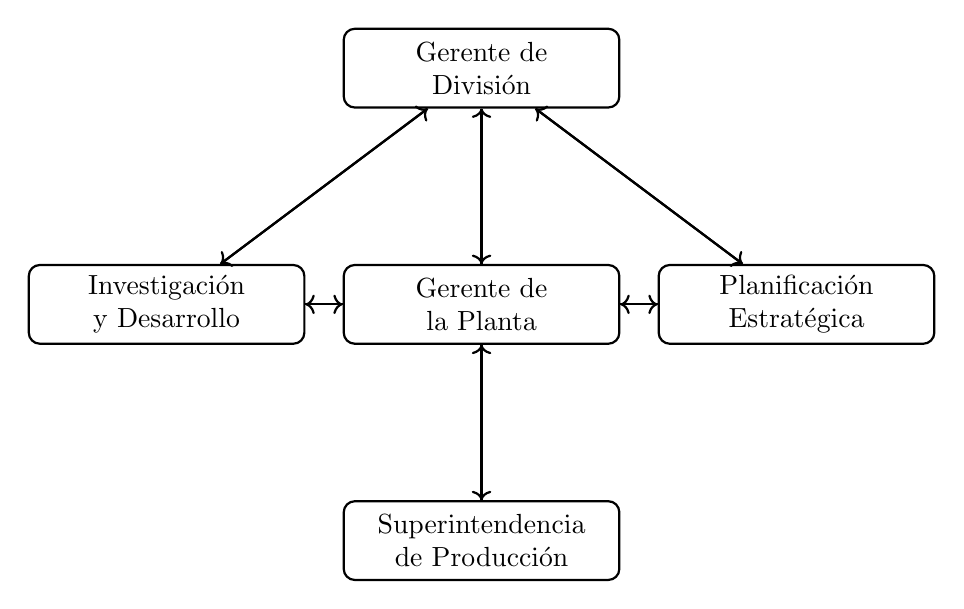
\begin{tikzpicture}[
        box/.style={draw, rounded corners, align=center, minimum width=3.5cm, minimum height=1cm, thick},
        arrow/.style={->, thick}
    ]
    % Nodos
    \node[box] (gerenteDivision) at (0, 3) {Gerente de \\ División};
    \node[box] (gerentePlanta) at (0, 0) {Gerente de \\ la Planta};
    \node[box] (investigacion) at (-4, 0) {Investigación \\ y Desarrollo};
    \node[box] (planificacion) at (4, 0) {Planificación \\ Estratégica};
    \node[box] (superintendencia) at (0, -3) {Superintendencia \\ de Producción};
    % Flechas
    \draw[arrow] (gerenteDivision) -- (gerentePlanta);
    \draw[arrow] (gerenteDivision) -- (investigacion);
    \draw[arrow] (gerenteDivision) -- (planificacion);

    \draw[arrow] (gerentePlanta) -- (gerenteDivision);
    \draw[arrow] (gerentePlanta) -- (superintendencia);
    \draw[arrow] (gerentePlanta) -- (investigacion);
    \draw[arrow] (gerentePlanta) -- (planificacion);

    \draw[arrow] (investigacion) -- (gerentePlanta);
    \draw[arrow] (investigacion) -- (gerenteDivision);

    \draw[arrow] (planificacion) -- (gerentePlanta);
    \draw[arrow] (planificacion) -- (gerenteDivision);

    \draw[arrow] (superintendencia) -- (gerentePlanta);

    \end{tikzpicture}
\end{center}

\subsection{Perfil de un proyecto}
\begin{itemize}
    \item Etapa mas preliminar de un proyecto.
    \item Análisis incluidos en esta etapa son de tipo estático.
    \item Se basa en información secundaria, generalmente, de tipo cualitativo (cifras estimativas y opiniones de expertos).
    \item Objetivo básico es \textbf{determinar si existen antecedentes que justifiquen abandonar el proyecto sin efectuar gastos futuros en estudios que buscan mayor y mejor profundidad.}
\end{itemize}

\subsection{Estudio de Prefactibilidad}

Se hacen proyecciones de costos y beneficios sobre la base decretorios cuantitativos. Esta es una etapa dinámica, ya que incorpora el factor del tiempo. Los beneficios y costos esperados para la vida del proyecto se estructuran en forma de flujos de caja.

\subsection{\hl{Resumen Evaluación del proyecto}}
\begin{enumerate}
    \item Se afinan los cálculos.
    \item Se incluye el equipamiento administrativo.
    \item Se incorpora la dotación del personal.
    \item Se define la capital de trabajo y se calcula el valor de desecho.
    \item Se incorporan todos los ingresos y egresos de caja atribuidos a la vida del proyecto.
    \item Se aplican las técnicas de evaluación que se consideren apropiadas.
\end{enumerate}

\subsection{Sensibilidad del proyecto}
Ya que es imposible predecir el futuro con 100\% de certeza, lo mas probable es que las variables consideradas en al evaluación registren cambios durante el desarrollo del proyecto.
Como complemento a la evaluación de un proyecto, se elaboran estudios de sensibilidad, estos consisten en mostrar el grado de variabilidad que puede resistir el proyecto.

Una de las formas de hacerlo es analizar que pasa con el VAN cuando se modifica alguna variable que pueda variar durante el periodo a evaluar. Teóricamente, se pueden hacer innumerables flujos, pero en la practica solo se confeccionan \textbf{tres}:
\begin{itemize}
    \item \textbf{Flujo inicial/normal:} Se basa en los datos originales.
    \item \textbf{Flujo optimista:} Se basa en los datos mas favorables.
    \item \textbf{Flujo pesimista:} Se basa en los datos menos favorables.
\end{itemize}
Todos estos flujos se realizan con valores en rangos realistas.

Otra de las maneras consiste en ver que tanto se puede modificar el valor de una variable considerada para la situación normal para que el proyecto mantenga su atractivo hacia el inversionista. A esto se le denomina \textbf{Modelo unidimensional}.

\subsubsection{Análisis de sensibilidad}
\begin{itemize}
    \item Modelos: Unidimensional, multidimensional.
    \begin{itemize}
        \item \textbf{Unidimensional:} Calcula el valor limite que puede tomar una variable, es decir, aquel que hace que el VAN sea igual a cero.
        \item \textbf{Hertz o multidimensional:} Mide que pasa con el van si cambia una o mas variables.
    \end{itemize}
\end{itemize}


\subsection{Sistema de evaluación de proyectos}

\begin{table}[H]
    \centering
    \renewcommand{\arraystretch}{1.5} % Ajusta este valor para cambiar la altura de las filas
    \begin{adjustbox}{max width=\textwidth}
        \begin{tabular}{|c|c|c|c|c|}
            \hline
            \multicolumn{5}{|c|}{\textbf{VIABILIDAD ECONÓMICA}} \\ \hline
            \multicolumn{4}{|c|}{\textbf{Formulación y preparación}} & \multicolumn{1}{c|}{\textbf{Evaluación}} \\ \hline
            \multicolumn{3}{|c|}{Obtención y creación de información} & {Flujo de caja} & {Evaluación Sensibilización} \\ \hline
            {Estudio mercado} & {Estudio organizacional} & {Estudio técnico} & \multicolumn{2}{c|}{Estudio financiero} \\ \hline
        \end{tabular}
    \end{adjustbox}
\end{table}

\newpage
\subsection{Estudio de mercado}

\subsubsection{Mercado competidor}
\begin{itemize}
    \item Precios que se cobran.
    \item Condiciones de crédito ofrecidas.
    \item Publicidad que se habrá que enfrentar.
    \item Diversidad de tamaño y tipos de envases.
    \item Promociones y regalos adicionales.
    \item Formas de llegar al consumidor.
    \item Competencia indirecta.
\end{itemize}

\textbf{Mercado competidor:}
\begin{itemize}
    \item \textbf{Indirecto:}
    \begin{itemize}
        \item \textbf{Compite por un proveedor o distribuidor.}
    \end{itemize}
    \item \textbf{Directo:}
    \begin{itemize}
        \item \textbf{Estrategia comercial.}
        \begin{itemize}
            \item Producto.
            \item Precio.
            \item Promoción.
            \item Plaza.
        \end{itemize}
        \item \textbf{Evolución del mercado.}
        \item \textbf{Éxitos y fracasos.}
    \end{itemize}
\end{itemize}

\subsubsection{Mercado proveedor}
\begin{itemize}
    \item Disponibilidad actual y potencial de insumos.
    \item Precios actuales y esperados.
    \item Condiciones de crédito de los proveedores.
    \item Políticas de descuento y plazo de entrega.
    \item Productos sustitutos.
    \item Características físicas que requiere el almacenamiento.
    \item Porcentaje del mercado que abarcara el proyecto.
\end{itemize}

\textbf{Mercado proveedor:}
\begin{itemize}
    \item \textbf{Precios.}
    \begin{itemize}
        \item Valor.
        \item Condiciones de crédito.
        \item Políticas de descuento.
    \end{itemize}
    \item \textbf{Disponibilidad.}
    \item \textbf{Calidad y especificaciones técnicas.}
\end{itemize}

\begin{tcolorbox}[colback=red!5!white,colframe=green!75!black]
    Suponga que proveedores locales venden un insumo a \$5.000 la unidad y existe la posibilidad de comprar a otro proveedor de otra localidad, que vende al mismo precio, pero el flete hace que el costo suba a \$5.500 por unidad. ¿Qué valor debe considerarse en el proyecto?

    \textbf{Respuesta:} Se debe considerar el valor de \$5.500, ya que es el valor real que se pagará por el insumo.
\end{tcolorbox}

\subsubsection{Mercado distribuidor}

\begin{itemize}
    \item Esta constituido por intermediarios.
    \item Costos de comercialización.
    \item Calidad del servicio
\end{itemize}

\textbf{Mercado proveedor:}
\begin{itemize}
    \item \textbf{Costo de intermediación.}
    \item \textbf{Calidad de servicio.}
    \item \textbf{Distribución propia o con intermediarios.}
\end{itemize}

\subsubsection{Mercado consumidor}
\begin{itemize}
    \item Consumidores actuales y potenciales de los productos del proyecto o de la competencia.
    \item El cliente emocional.
    \item Distorsiones en proyección de la demanda.
\end{itemize}

\subsubsection{Tecnicas de proyeccion de demanda}
\vspace{0.5cm}
\begin{center}
    \begin{minipage}[H]{0.45\textwidth}
        \begin{itemize}
            \item \textbf{Métodos cualitativos} 
            \begin{itemize}
                \item Opiniones de expertos.
                \item Investigación de mercados.
                \begin{itemize}
                    \item Encuestas de intenciones de compra.
                \end{itemize}
            \end{itemize}
        \end{itemize}
    \end{minipage}
    \hfill
    \begin{minipage}[H]{0.45\textwidth}
        \begin{itemize}
            \item \textbf{Modelos de series temporales}
            \begin{itemize}
                \item Regresión f(t).
                \item Promedios móviles.
            \end{itemize}
            \item \textbf{Métodos causales}
            \begin{itemize}
                \item Regresión f(v).
                \item Modelos econométricos.
            \end{itemize} 
        \end{itemize}
    \end{minipage}
\end{center}

\subsubsection{Regresión simple}
Este es de los métodos mas utilizados para proyectar la demanda, ya que es fácil de entender y aplicar. Su formula es:
\begin{equation*}
    y = a + bx
\end{equation*}

\textit{Donde:}

\begin{align*}
    b = \frac{n(\sum xy) - (\sum x)(\sum y)}{n(\sum x^2) - (\sum x)^2} \\
\end{align*}

\textit{y:}

\begin{equation*}
    a = \overline{y} - b\overline{x}
\end{equation*}

\begin{tcolorbox}[colback=red!5!white,colframe=blue!75!black]
    Considere la siguiente tabla de datos;

    \begin{table}[H]
        \centering
        \begin{tabular}{|c|c|c|}
            \hline
            Observac. & Pobl. Infantil (miles) x & Ventas (y) \\\hline
            1 & 14.68 & 3,845 \\\hline
            2 & 22.93 & 5,450 \\\hline
            3 & 16.65 & 5,099 \\\hline
            4 & 35.99 & 8,890 \\\hline
            5 & 32.48 & 6,681 \\\hline
            6 & 38.77 & 9,678 \\\hline
            7 & 10.03 & 4,542 \\\hline
            8 & 24.26 & 4,557 \\\hline
            9 & 52.46 & 13,289 \\\hline
            10 & 36.80 & 10,506 \\\hline
            11 & 17.34 & 5,134 \\\hline
            12 & 43.69 & 9,066 \\\hline
        \end{tabular}
    \end{table}

    Calcule el nivel de ventas que habría si la población infantil fuera de 45.000 habitantes.

    \textbf{Respuesta:} Para calcular el nivel de ventas, primero se debe calcular el valor de $a$ y $b$.

    \begin{align*}
        % \sum xy &= (14,66*3845) + (22,93*5450) + (16,65 * 5099) + (35,99*8890) + (32,48 * 6681) + (38,77 * 9678) + (10,03 * 4542) + (24,26 * 4557) + (52,46 * 13289) + (36,80 * 10506) + (17,34 * 5134) + (43,69 * 9066) = 2903388,51 \\
        \sum xy &= (14,66*3845) + (22,93*5450) + \cdots + (43,69 * 9066) = 2903388,51 \\
        % \sum x &= 14.68+22.93+16.65+35.99+32.48+38.77+10.03+24.26+52.46+36.80+17.34+43.69 = 346,08 \\
        \sum x &= 14.68+22.93+16.65+\cdots+43.69 = 346,08 \\
        % \sum x^2 &= 14.68^2 + 22.93^2 + 16.65^2 + 35.99^2 + 32.48^2 + 38.77^2 + 10.03^2 + 24.26^2 + 52.46^2 + 36.80^2 + 17.34^2 + 43.69^2 = 11876,785 \\
        \sum x^2 &= 14.68^2 + 22.93^2 + \cdots + 43.69^2 = 11876,785 \\
        % \sum y &= 3845+5450+5099+8890+6681+9678+4542+4557+13289+10506+5134+9066 = 86737 \\
        \sum y &= 3845+5450+\cdots+9066 = 86737 \\
        \\
        b &= \frac{12(2903388,51)- (346,08)(86737)}{12(11876,785) - (346,08)^2}\\
        b &= 211,987243\\
        \\
        a &= \frac{86737}{12} - 211,987243 * \frac{346,08}{12} \\
        a &= 1114,371245
    \end{align*}
    Por lo tanto, las ventas estimadas para una población de 45.000 habitantes son:
    \begin{align*}
        y &= 1114,371245 + 211,987243 * 45 \\
        y &= 10653,79718 \\
        y &\approx \$10653,80
    \end{align*}   
\end{tcolorbox}

\subsubsection{El mercado del proyecto}
\vspace{1.5cm}
\begin{center}
    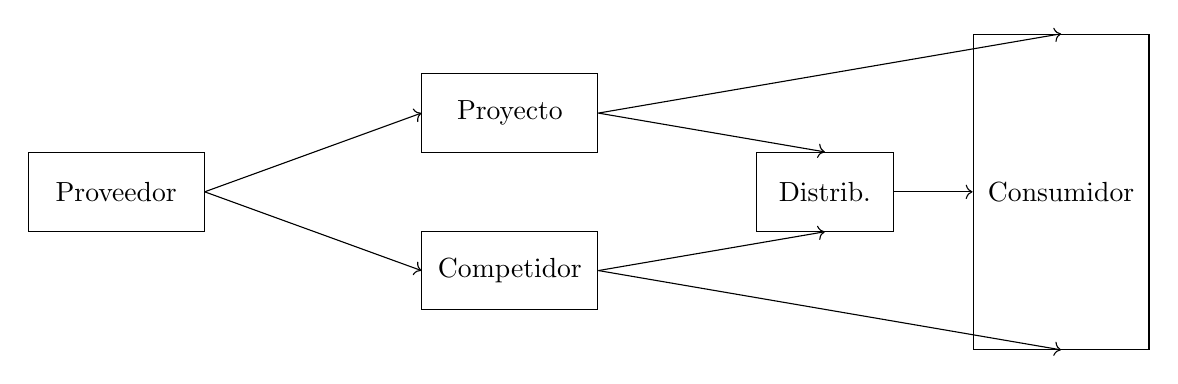
\begin{tikzpicture}
        % Proveedor
        \node[draw, rectangle, minimum width=1cm, minimum height=1cm, text width=2cm, align=center] (proveedor) at (0,0) {Proveedor};
        
        % Proyecto
        \node[draw, rectangle, minimum width=2cm, minimum height=1cm, text width=2cm, align=center] (proyecto) at (5,1) {Proyecto};
        
        % Competidor
        \node[draw, rectangle, minimum width=2cm, minimum height=1cm, text width=2cm, align=center] (competidor) at (5,-1) {Competidor};
        
        % Distribuidor
        \node[draw, rectangle, minimum width=1cm, minimum height=1cm, text width=1.5cm, align=center] (distrib) at (9,0) {Distrib.};
        
        % Consumidor
        \node[draw, rectangle, minimum width=1cm, minimum height=4cm, text width=2cm, align=center] (consumidor) at (12,0) {Consumidor};
        
        % Arrows
        \draw[->] (proveedor.east) -- (proyecto.west);
        \draw[->] (proveedor.east) -- (competidor.west);
        \draw[->] (proyecto.east) -- (distrib.north);
        \draw[->] (proyecto.east) -- (consumidor.north);
        \draw[->] (competidor.east) -- (distrib.south);
        \draw[->] (competidor.east) -- (consumidor.south);
        \draw[->] (distrib.east) -- (consumidor.west);
    \end{tikzpicture}
\end{center}

\subsubsection{Objetivos del estudio de mercado}
El estudio de marcado se hace para cumplir con una variedad de objetivos, dentro de los cuales están:
\begin{itemize}
    \item Confirmar la existencia de una necesidad insatisfecha en el mercado o la necesidad de ofrecer un mejor servicio.
    \item Determinar la cantidad de bienes-servicios adicionales que la comunidad estaría dispuesta a adquirir, dado un precio.
    \item Conocer los medios para llegar al consumidor o usuario.
    \item Obtener una idea sobre el riesgo de que el bien o servicio no sea aceptado en el mercado.
\end{itemize}

\subsubsection{Resultados del estudio de mercado}
\begin{itemize}
    \item Análisis de la oferta.
    \item Análisis de la demanda.
    \item Análisis de los precios.
    \item Análisis de la comercialización.
    \item Conclusiones del estudio de mercado.
\end{itemize}

\subsection{Proyectos de Outsourcing (Profesor Sapag) [Resumen]}

Los proyectos de \textit{outsourcing} han ganado relevancia en los últimos años, ya que permiten a las empresas mejorar la rentabilidad de su gestión mediante la externalización de actividades no esenciales. Entre las principales ventajas del \textit{outsourcing} se incluyen:
\begin{itemize}
    \item Focalización en el giro principal de la empresa.
    \item Mitigación de riesgos compartiendo inversiones con proveedores externos.
    \item Liberación de recursos para otras actividades rentables.
    \item Mejora en la eficiencia al transferir tareas especializadas a expertos.
    \item Acceso a tecnologías avanzadas sin necesidad de grandes inversiones.
    \item Apoyo en estrategias de crecimiento al suplir deficiencias en servicios.
\end{itemize}

El \textit{outsourcing} también contribuye a reducir distracciones operativas, permitiendo a las empresas concentrarse en mejorar la calidad, rapidez y precisión de sus procesos.

Sin embargo, presenta desventajas como:
\begin{itemize}
    \item Pérdida de control sobre actividades externalizadas.
    \item Dependencia de terceros y riesgo en la transferencia de información.
    \item Posibles costos externos elevados debido a utilidades y transportes.
    \item Pérdida de talentos internos especializados.
\end{itemize}

Para una correcta evaluación, se deben considerar no solo los costos contables, sino también los costos reales y los efectos fiscales, de depreciación y de gestión. Además, los flujos de caja deben reflejar tanto los ingresos por la venta de activos como los efectos impositivos asociados.

\subsection*{Ejemplo de Evaluación de Proyecto de Outsourcing}

La empresa XYZ está evaluando la conveniencia de externalizar el servicio de mantenimiento de su maquinaria. Actualmente, este servicio tiene un costo de \$14,000 anuales. La externalización implicaría un costo de \$18,200 anuales al proveedor externo, pero permitiría vender la maquinaria hoy en \$13,000, cuyo valor en libros es de \$12,000 y con dos años restantes de depreciación. Sin externalización, la maquinaria podría usarse durante cuatro años más y venderse en \$6,000 al final de ese periodo. Se considera una tasa de impuesto a las utilidades del 17\% y una tasa de descuento del 12\%.

\subsubsection*{Flujo de Caja del Outsourcing}

El flujo de caja incremental para la opción de outsourcing incluye:

\begin{itemize}
    \item Costo de servicio anual de outsourcing: \$18,200.
    \item Venta del activo en el momento inicial (momento 0): \$13,000.
    \item Valor en libros del activo: \$12,000.
    \item Valor de desecho en cuatro años (sin outsourcing): \$6,000.
    \item Tasa de impuesto: 17\%.
\end{itemize}

\subsubsection*{Cálculo de Depreciación y Efecto Tributario}

La depreciación anual restante del activo es:
\[
\text{Depreciación Anual} = \frac{12,000}{2} = 6,000
\]
El ahorro fiscal por depreciación en caso de mantener el activo internamente sería:
\[
\text{Ahorro Tributario} = 6,000 \times 0.17 = 1,020
\]

\subsubsection*{Flujo de Caja Incremental del Outsourcing}

\begin{table}[H]
    \centering
        \begin{tabular}{lrrr}
            \toprule
            \textbf{Concepto} & \textbf{Año 0} & \textbf{Años 1-3} & \textbf{Año 4} \\
            \midrule
            Costo del servicio de outsourcing &  & -18,200 & -18,200 \\
            Venta del activo & 13,000 &  & -6,000 \\
            Ahorro por depreciación &  & 1,020 &  \\
            Efecto impositivo sobre venta (valor contable: \$12,000) & 170 &  &  \\
            \midrule
            \textbf{Flujo de Caja} & 13,170 & -17,180 & -24,200 \\
            \bottomrule
        \end{tabular}
    \caption{Flujo de Caja Incremental con Outsourcing}
\end{table}

\subsubsection*{Cálculo del VAN}

El VAN se calcula descontando los flujos de caja a una tasa del 12\%.

\[
\text{VAN} = \frac{13,170}{(1 + 0.12)^0} + \frac{-17,180}{(1 + 0.12)^1} + \frac{-17,180}{(1 + 0.12)^2} + \frac{-24,200}{(1 + 0.12)^3}
\]

Calculando cada término:

\[
\text{VAN} = 13,170 - 15,339.29 - 13,697.00 - 17,541.02 = -2,752.31
\]

\subsubsection*{Conclusión}

Dado que el VAN es negativo (\$-2,752.31), no es conveniente externalizar el servicio de mantenimiento de maquinaria.

\subsection{Determining the Right Price for a Product or Service [Resumen]}

\subsubsection*{Introducción}
La fijación de precios es fundamental tanto en los aspectos financieros como en los de marketing. El precio de un producto o servicio debe cubrir costos, generar beneficios y evitar precios excesivos que puedan alienar a los clientes. Este artículo aborda consideraciones clave al establecer precios.

\subsubsection*{Elementos Clave en la Determinación del Precio}

\begin{itemize}
    \item \textbf{Calculo de costos}: Se debe calcular el costo mínimo unitario y luego investigar el precio máximo que el mercado podría aceptar, estableciendo el precio final entre ambos.
    \item \textbf{Comparación con la competencia}: Bajar el precio no siempre es la mejor estrategia para ganar mercado. Las pequeñas empresas pueden destacar con un mejor servicio, calidad o entrega rápida.
    \item \textbf{Ajustes de precios}: En ocasiones, se requiere un aumento de precio para cubrir costos adicionales. Es importante comunicar estos cambios a los clientes para mantener una buena relación.
    \item \textbf{Flexibilidad de precios}: La posibilidad de ajustar precios depende de la estrategia del producto en el mercado. Una estrategia de diferenciación permite una mayor flexibilidad que una de liderazgo en costos.
    \item \textbf{Ofrecimiento gratuito}: Proporcionar muestras gratuitas puede atraer clientes, especialmente si se pueden diferenciar los productos de la competencia.
\end{itemize}

\subsubsection*{Estrategias de Precios}

\begin{itemize}
    \item \textbf{Precios basados en costos}: Se calcula el costo total y se agrega un margen de beneficio.
    \item \textbf{Precios de desnatado}: Precio inicial alto para recuperar costos rápidamente, bajando el precio si entran competidores.
    \item \textbf{Precios negociados}: El precio se ajusta según las cantidades compradas.
    \item \textbf{Precio esperado}: Basado en la percepción del cliente de que el producto es “el mejor”.
    \item \textbf{Precios diferenciales}: Ofrecer distintos precios a distintos segmentos de mercado, como descuentos a clientes leales o precios especiales en temporadas bajas.
    \item \textbf{Precio de por vida}: Se justifica un precio inicial más alto demostrando menores costos de mantenimiento a largo plazo.
\end{itemize}

\subsubsection*{Errores Comunes}

\begin{itemize}
    \item \textbf{Precios demasiado bajos}: Competir solo en precio es riesgoso, especialmente para las pequeñas empresas. La diferenciación es clave.
    \item \textbf{Precios altos sin suficiente volumen de ventas}: El precio debe cubrir los costos y generar ganancias. Si no se alcanzan los volúmenes proyectados, deben tomarse medidas correctivas.
    \item \textbf{Estructuras de precios demasiado simples}: El precio debe formar parte de una estrategia de marketing bien investigada, que incluya un análisis del mercado y de la competencia.
\end{itemize}

\begin{tcolorbox}[title=Lecturas Adicionales]
    \begin{itemize}
        \item \textbf{Libro}: Mohammed, Rafi. \textit{The Art of Pricing: How to Find the Hidden Profits to Grow Your Business}. Nueva York: Crown, 2005.
        \item \textbf{Sitio Web}: \textit{Professional Pricing Society}: \href{www.pricingsociety.com}{www.pricingsociety.com}
    \end{itemize}
\end{tcolorbox}

\subsection{Estudio técnico}
Algunos evaluadores consideran esta como la etapa mas simple en la evaluación de proyectos, ya que entienden que la responsabilidad es de los técnicos e ingenieros, sin embargo, parta obtener un resultado viable, un buen evaluador debe tener la capacidad de compenetrarse con los aspectos técnicos del proyecto.

Se debe tomar en cuenta que existen ocasiones en que algunos técnicos, con el fin de que se aprueben sus proyectos, omitan o minimicen ciertos aspectos relevantes relacionados a su rama.

Teniendo todo esto en cuenta, el evaluador puede cumplir con su obligación de buscar soluciones alternativas que mejoren los resultados financieros del proyecto.
\begin{itemize}
    \item Inversiones en obras físicas.
    \item inversiones en equipamiento.
    \item Aspectos técnicos propios del proyecto.
    \item Costos de operación.
    \begin{itemize}
        \item Materias primas, insumos y materiales.
        \item Recursos humanos.
        \item Servicios.
        \item Curva de aprendizaje.
        \item Uso de estándares.
    \end{itemize}
\end{itemize}

\subsubsection{Inversiones en obras físicas}
\vspace{0.5cm}
\begin{minipage}[H]{0.45\textwidth}
    \begin{itemize}
        \item Terrenos.
        \item Metros de edificación.
        \item Tipo de construcción.
        \item Instalaciones adicionales (1).
        \begin{itemize}
            \item Accesos y estacionamientos.
        \end{itemize}
    \end{itemize}
\end{minipage}
\hfill
\begin{minipage}[H]{0.45\textwidth}
    \begin{itemize}
        \item Instalaciones adicionales (2).
        \begin{itemize}
            \item Romanas para los caminos.
            \item Disposición de desechos.
        \end{itemize}
        \item Costos de mantención.
        \begin{itemize}
            \item Despejes periódicos.
        \end{itemize}
    \end{itemize}
\end{minipage}


\subsubsection{Inversiones en equipamiento}
\vspace{0.5cm}
\begin{minipage}[H]{0.45\textwidth}
    \begin{itemize}
        \item Listado de maquinarias y equipos.
        \begin{itemize}
            \item Grúas y montacargas.
            \item Pesómetros, flujómetros, etc.
        \end{itemize}
        \item Mobiliario.
    \end{itemize}
\end{minipage}
\hfill
\begin{minipage}[H]{0.45\textwidth}
    \begin{itemize}
        \item Equipos de oficina.
        \begin{itemize}
            \item Aire acondicionado.
            \item PC's, copiadoras, etc.
        \end{itemize}
        \item Vehículos.
    \end{itemize}
\end{minipage}

En estas inversiones existen algunos aspectos que se deben considerar, como:
\begin{itemize}
    \item El costo debe justificarse, de preferencia, con cotizaciones.
    \item Se debe considerar la depreciación de los equipos, con el fin de establecer programas de reemplazo y para correcto cómputo de depreciación.
    \item Precio de venta de los equipos que se reemplazan.
    \item Costos de mantención de los equipos. 
\end{itemize}

\subsubsection*{Inversiones}
\vspace{0.5cm}
\begin{minipage}[H]{0.45\textwidth}
    \begin{itemize}
        \item \textbf{Previas a la puesta en marcha.}
        \begin{itemize}
            \item Construcciones.
            \item Equipamiento.
            \item \textcolor{blue}{Promoción.}
            \item \textcolor{blue}{Sistemas de información.}
            \item \textcolor{orange}{Estudios.}
            \item \textcolor{orange}{Gastos.}
            \item \textcolor{orange}{Capital de trabajo.}
        \end{itemize}
    \end{itemize}
\end{minipage}
\hfill
\begin{minipage}[H]{0.45\textwidth}
    \begin{itemize}
        \item \textbf{Durante la operación.}
        \begin{itemize}
            \item Por ampliación.
            \item Por reemplazo.
        \end{itemize}
    \end{itemize}
\end{minipage}

\subsubsection*{Vida util de los activos}
\vspace{0.5cm}
\begin{center}
    \begin{minipage}[H]{0.5\textwidth}
        \begin{itemize}
            \item Contable.
            \item Técnica.
            \item Comercial.
            \item Económica.
        \end{itemize}
    \end{minipage}
\end{center}

\subsubsection{Costos de operación}
El estudio técnico genera información importante y relevante para determinar los costos que existirán en la operación del proyecto. De estos costos es básico determinar cuales serán \textbf{fijos} y cuales serán \textbf{variables}.

Durante el proceso es normal que se presenter perdidas, sin embargo, estas deben ser consideradas como parte del proceso de aprendizaje y no como un fracaso. Estas perdidas se conocen como \textit{perdidas de insumos} que representan evaporaciones, descartes o filtraciones.

\subsubsection*{Costos de recursos humanos}
\begin{itemize}
    \item Por cada área productiva.
    \item Por cada área administrativa.
    \item Por cada área de comercialización.
    \item La idea es predeterminar el gasto que se tendrá por concepto de remuneraciones y costos anexos.
    \item \hl{¿De donde se obtiene el dato de sueldos por cada cargo?} 
\end{itemize}
\subsubsection*{Costos de los servicios}
\begin{itemize}
    \item Arriendo de camiones.
    \item Arriendo de maquinaria y equipos.
    \item Arriendo de vehículos.
    \item Movimiento de tierras.
    \item Casino.
    \item Servicios de seguridad y medioambientales.
    \item Transporte de carga.
    \item Transporte de personal.
\end{itemize}

\subsubsection{Objetivos del estudio técnico}
Dentro de los objetivos de este estudio se encuentra el \textbf{verificar la posibilidad técnica de la fabricación del producto que se pretende elaborar}. 
Ademas de esto se busca \textbf{analizar y determinar}: localización optima, tamaño optimo, equipos necesarios, instalaciones y organización requeridos para realizar la producción. 

\subsubsection{Contenido del estudio técnico}
\begin{itemize}
    \item Localización óptima de la planta.
    \item Determinación de la capacidad instalada y óptima de la planta.
    \item Descripción del proceso productivo.
    \item Selección de equipos y maquinarias.
    \item Cálculo de la mano de obra necesaria.
    \item Justificación de la cantidad de equipo requerida.
    \item Pruebas de control de calidad.
    \item Mantenimiento que se aplicará.
    \item Determinación de las áreas de trabajo necesarias.
    \item Análisis de la disponibilidad y el costo de materias primas, materiales e insumos.
    \item Distribución de planta.
    \item Costos.
    \item Conclusiones del estudio técnico.
\end{itemize}

\newpage
\subsection{Valor del desecho (Profesor Sapag) [Resumen]}

\subsubsection*{Introducción}
La evaluación de proyectos no debe considerarse simplemente como una técnica de toma de decisiones, sino como una herramienta informativa para apoyar dicho proceso. Con frecuencia, una misma evaluación puede llevar a decisiones opuestas dependiendo del inversionista y sus circunstancias individuales, tales como sus estrategias de negocio, expectativas o su percepción sobre la validez de los datos provistos.

\subsubsection*{La Responsabilidad del Evaluador}
El papel del evaluador es fundamental para la precisión del análisis. Un uso inadecuado de conceptos o técnicas puede llevar a decisiones incorrectas. Existen prácticas comúnmente aceptadas sin cuestionar su validez en casos específicos, como la recuperación del capital de trabajo al final del horizonte de evaluación o la reposición de activos que coinciden con dicho horizonte.

\subsubsection*{Métodos de Cálculo del Valor de Desecho}
El valor de desecho o remanente al final del horizonte de evaluación puede calcularse mediante tres métodos distintos:

\begin{itemize}
    \item \textbf{Valor Contable}: Basado en el valor en libros, donde los activos se deprecian según el sistema contable.
    \item \textbf{Valor Comercial}: Determinado por el valor de mercado de los activos.
    \item \textbf{Valor Económico o Flujo Perpetuo}: Calcula el valor actual de los flujos que los activos pueden generar indefinidamente, restando una reserva para la reposición de activos.
\end{itemize}

\textbf{Flujos Perpetuos:}
El cálculo del flujo perpetuo adecuado es esencial en proyectos productivos. La fórmula clásica para una perpetuidad en finanzas es:

\begin{equation}
    VA = \frac{F}{r}
\end{equation}

sin embargo, esta ecuación no es aplicable en proyectos productivos, donde es necesario considerar una reserva de reposición. La fórmula adecuada es:

\begin{equation}
    VA = \frac{F - RR}{r}
\end{equation}

donde $RR$ es la reserva de reposición, calculada como la depreciación real o contable de los activos.

\subsubsection*{Prácticas de Evaluación en el Flujo de Caja}
Dos prácticas en la construcción de flujos de caja dependen del método de cálculo del valor de desecho:

\textbf{Reposición de Activos al Final del Horizonte de Evaluación:}
Al finalizar el horizonte, la reposición debe incluirse para mantener la capacidad productiva, particularmente si se emplea el método económico. En los métodos de valoración de activos, esta reposición es indiferente.

\textbf{Recuperación del Capital de Trabajo:}
En el valor contable y comercial, la recuperación del capital de trabajo siempre debe incluirse, pues es un activo del inversionista. En el valor de flujo, esta recuperación no debe incluirse ya que el capital de trabajo es necesario para generar flujos futuros.

\begin{table}[H]
    \centering
    \renewcommand{\arraystretch}{1.5} % Ajusta este valor para cambiar la altura de las filas
    \begin{tabularx}{\textwidth}{|>{\centering\arraybackslash}X|>{\centering\arraybackslash}X|>{\centering\arraybackslash}X|}
        \hline
        \textbf{} & \textbf{Recuperación del Capital de Trabajo} & \textbf{Reposición de Activos al Final del Horizonte de Evaluación} \\
        \hline
        \textbf{Valor de los Activos} & \textcolor{darkorange}{\textbf{SIEMPRE}} debe incluirse la recuperación al final del horizonte de evaluación porque es un activo más de propiedad del inversionista. & Es \textcolor{darkorange}{\textbf{INDIFERENTE}} incluir o no la reposición al final del horizonte de evaluación, porque el mayor valor de desecho se anula con el valor de la inversión. \\
        \hline
        \textbf{Valor del Flujo} & \textcolor{darkorange}{\textbf{NUNCA}} debe incluirse la recuperación al final del horizonte de evaluación porque es necesario disponer de él para generar los flujos futuros. & \textcolor{darkorange}{\textbf{SIEMPRE}} debe incluirse la reposición al final del horizonte de evaluación, para permitir seguir generando los flujos futuros. \\
        \hline
    \end{tabularx}
    \caption{Consideraciones para la Recuperación del Capital de Trabajo y la Reposición de Activos}
\end{table}

\subsubsection*{Conclusión}
La discusión sobre estos temas evidencia la importancia de aplicar criterios específicos y evaluar cada elemento del flujo de caja de acuerdo con las particularidades del proyecto. La teoría debe ser adaptada al contexto específico para evitar errores en la toma de decisiones de inversión.


\end{document}
